\documentclass[10pt, oneside]{article} 
\usepackage{amsmath, amsthm, amssymb, calrsfs, wasysym, verbatim, bbm, color, graphics, graphicx, geometry}
\usepackage[most]{tcolorbox}
\usepackage{xcolor}
\usepackage{framed}
\colorlet{shadecolor}{blue!15}
\graphicspath{ {./} }

\geometry{tmargin=.75in, bmargin=.75in, lmargin=.75in, rmargin = .75in}  

\newcommand{\R}{\mathbb{R}}
\newcommand{\C}{\mathbb{C}}
\newcommand{\Z}{\mathbb{Z}}
\newcommand{\N}{\mathbb{N}}
\newcommand{\Q}{\mathbb{Q}}
\newcommand{\Cdot}{\boldsymbol{\cdot}}

\newtheorem{thm}{Theorem}
\newtheorem{defn}{Definition}
\newtheorem{conv}{Convention}
\newtheorem{rem}{Remark}
\newtheorem{lem}{Lemma}
\newtheorem{cor}{Corollary}
\newtheorem{exa}{Example}


\title{Clase \# 3: Presion y estatica de los fluidos} 
\author{\textbf{Luis Alejandro Morales}\\ \vspace{0.4cm} Profesor Asistente \\ Universidad Nacional de Colombia-Bogot\'a\\Facultad de Ingenier\'ia \\ Departamento de Ingenieria Civil y Agr\'icola}
\date{Periodo 2022-II}

\begin{document}

\maketitle
\tableofcontents

\vspace{.25in}


\section{Presi\'on}
En mecanica de fluidos, la \textbf{presi\'on} es definida como la fuerza normal ejercida por un fluido por unidad de area. En otras areas, la presion ejercida sobre un solido se conoce como el \textbf{esfuerzo normal}. En SI, las unidades de la presi\'on  son el \textbf{pascal}(Pa) donde $1\ Pa = 1\ N/m^2$. Otras unidades de presion usadas comunmente son:
\begin{flalign*}
1\ bar\ &=\ 10^5\ Pa\ =\ 0.1\ MPa\ =\ 100\ kPa \\
1\ atm\ &=\ 101325\ Pa\ =\ 101.325\ kPa\ =\ 1.01325\ bars \\
1\ kgf/cm^2 \ &=\ 9.807\ N/cm^2\ =\ 9.807E4\ N/m^2\ =\ 9.807E4\ Pa \\
&=\ 0.9807\ bar \\
&=\ 0.9679\ atm 
\end{flalign*}

En sistema ingles, las unidade de la presi\'on son libra fuerza por puldaga cuadrada ($lbf/in^2$ o $psi$). Algunas equivalencias entre los dos sistemas son:
\begin{flalign*}
1\ atm\ &=\ 14.696\ psi \\
1\ kgf/cm^2 \ &=\ 14.223\ psi 
\end{flalign*}

Algunas definiciones son:
\begin{itemize}
\item \textbf{presion absoluta} $P_{abs}$: Es la presion actual sobre un cuerpo y es medida con respecto al vacio absoluto (presion cero). La mayoria de los medidores de presion son calibrados para medir la presion tomando como cero la presi\'on atmosferica local.
\item \textbf{presion de manometro} $P_{gage}$: Es la diferencia entre la presion absoluta y la presion atmosferica local. 
\item \textbf{presion de vacio} $P_{vac}$: Se presenta cuando una presion esta por debajo de la presion atmosferica ($P_{gage}<0$). 
\end{itemize}

La relacion entre estas presiones es (ver figura~\ref{pres1}):
\begin{equation}
P_{gage} = P_{abs}-P_{atm}
\end{equation}

\begin{equation}
P_{vac} = P_{atm}-P_{abs}
\end{equation}

% Fig 3.3 Cengel
\begin{figure}[h]
\centering
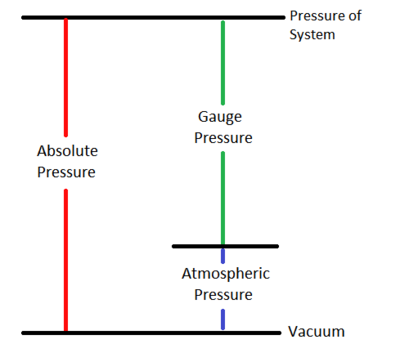
\includegraphics[width=10cm]{pres1}
\caption{Presi\'on atmosferica, de manometro y de vacio}
\label{pres1}
\end{figure}

Es comun encontrar por ejemplo que la presion de manometro tipica de una llanta de un carro es 32.0 $psi$, la cual es tomada con respecto a la presion atmosferica. Si la presion atmosferica en el sitio en donde se encuentra el carro es de 14.3 $psi$, la presion absoluta seria $32.0\ +\ 14.3\ =\ 46.3\ psi$. Note que en algunos problemas las unidades $psig$ hacen referencia a presion de manometro mientras que las unidades $psia$ hacen referencia a presion absoluta. 

\subsection{Presi\'on en un punto}
Por definicion, la presion en un punto en un fluido es la misma en todas las direcciones, por lo tanto la presion no puede considerarse como una cantidad vectorial y es entonces una cantidad scalar. Esto se puede demostrar si se hace un analisis de fuerzas sobre el elemento en equilibrio de la figura~\ref{ppoint} en donde la profundidad del elemento es $\Delta y = 1$. Aplicando la segunda ley de Newton y haciendo un analisis de fuerzas sobre las superficies del elemento:

\begin{equation}
\begin{split}
\sum F_x &= ma_x = 0: \quad P_1 \Delta y \Delta z - P_3 \Delta y l \sin \theta = 0 \\
\sum F_z &= ma_z = 0: \quad P_2 \Delta y \Delta x - P_3 \Delta y l \cos \theta - \frac{1}{2}\rho g \Delta x \Delta y \Delta z = 0
\label{ppo}
\end{split}
\end{equation}

donde $\rho$ es la densidad y $W = mg = \frac{1}{2} \rho g \Delta x \Delta y \Delta z$ es el peso del elemento. Teniendo en cuenta que $\Delta x = l \cos \theta$ y $\Delta z = l \sin \theta$, reemplazando en la ecuacion~\ref{ppo} y simplificando:

\begin{equation}
\begin{split}
P_1 - P_3 = 0 \\
P_2 - P_3 - \frac{1}{2}\rho g \Delta z = 0
\label{ppo1}
\end{split}
\end{equation}
El ultimo termino de la ecuaci\'on~\ref{ppo1} se elimina teniendo en cuenta que cuando el elemento se vulve infinitesimal y se reduce a un punto $\Delta z \rightarrow 0$. Por tanto:

\begin{equation}
\begin{split}
P_1 = P_2 = P_3 = P
\label{ppo2}
\end{split}
\end{equation}

Con esto concluimos que la presion $P$ en un punto en un fluido tiene la misma magnitud en todas las direcciones. Esto se aplica para un fluido en moviento o en reposo teniendo en cuenta que la presion es un escalar. 

\subsection{Variaci\'on de la presi\'on con la profundidad}
Es conocido que la presion de un fluido en reposo no cambia en direccion horizontal y su cambio es en direccion vertical. Por esto, la presion en un fluido incrementa con la profundidad ya que este incremento implica mayor cantidad de fluido y por tanto mayor peso lo cual es balanceado con un incremento de la presi\'on.

Para obtener una relacion de la variaci\'on de la presion con la profundidad, analicemos las fuerzas actuantes sobre el elemento en equilibrio de la figura~\ref{pres2} cuya profundidad es $\Delta y =1$. 

% Fig 3.7 Cengel
\begin{figure}[h]
\centering
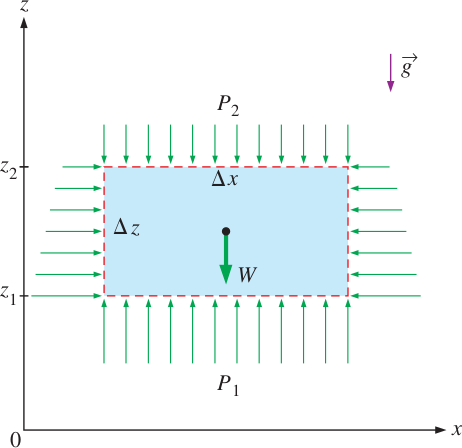
\includegraphics[width=10cm]{pres2}
\caption{Diagrama de cuerpo libre de un elemento rectangular de fluido en equilibrio.}
\label{pres2}
\end{figure}

Asumiendo que la densidad $\rho$ del fluido es constante, el balance de fuerzas en la direccion $z$ es:
$$
\sum F_z = m a_z = 0: \quad P_1 \Delta x \Delta y - P_2 \Delta x \Delta y - \rho g \Delta x \Delta y \Delta z = 0
$$
donde $W = mg = \frac{1}{2} \rho g \Delta x \Delta y \Delta z$ es el peso del elemento y $\Delta z = z_2 - z_1 $. Dividiendo por $\Delta x \Delta y$, tenemos:

\begin{equation}
\Delta P = P_2 - P_1 = -\rho g \Delta z = -\gamma_s \Delta z
\label{ppr1}
\end{equation}

donde $\gamma_s = \rho g$ es el peso especifico  del fluido. Otra manera de expresar la ecuacion~\ref{ppr1}anterior es:

\begin{equation}
\Delta P_{below} = P_{above} + \gamma_s |\Delta z|
\label{ppr2}
\end{equation}

donde "below" indica el punto mas bajo mientras que "above" indica el punto mas alto. Debido a que la densidad de los gases $\approx\ 0$, por ejemplo, la presion en una habitacion es uniforme ya que el peso del gas es muy bajo por lo que la ecuacion~\ref{ppr1} se convierte en $\Delta P=0$. 
Si tomamos el punto "above" sobre la superficie de el liquido a superficie abierta, cuya presion es la atmosferica $P_{atm}$, la presion a una profundidad $h$ (medida desde la superficie), la presion es:

\begin{equation}
P = P_{atm} + \rho g h \quad \text{or} P_{gage}=\rho g h
\label{ppr3}
\end{equation}

Como los fluidos son esencialmente inconpresibles, la variaci\'on de $\rho$ es despreciable con respecto a la profundidad. Cuando se requiere una alta precision en el calculo de $P$  debido a cambios fuertes de temperature en fluidos, es necesario saber como $\rho$ cambia con la temperatura. Ademas, cuando se requiere calcular  $P$ a grandes profundidades en el oceano, es importante determinar como cambia a la densidad con la profundidad.

Para fluidos cuya densidad cambia significantemente con la elevacion, una relacion de la variacion de la presion con respecto a la elevacion es obtenida dividiendo la ecuacion~\ref{ppr1} por $\Delta z \rightarrow 0$, es:

\begin{equation}
\frac{dP}{dz} = -\rho g
\label{ppr4}
\end{equation}

Noten que $dP$ es negativa cuando $dz$ es positiva teniendo en cuenta que la presion decrease hacia arriba.Si $\rho$ es conocida con la elevacion, la diferencia de presion entre dos puntos 1 y 2 (ver figura~\ref{pres2} se determina como:

\begin{equation}
\Delta P = P_2 - P_1 = -\int_1^2 \rho g dz
\label{ppr5}
\end{equation}

Como lo habiamos mencionado anteriormente, en un fluido en reposo la presion sobre cualquier tipo de superficie cambia unicamente con la profundidad. En la figura~\ref{pres3} vemos que la presion en los puntos A, B, C, D, E, F y G sobre superficies de diferentes formas es la misma, ya que estan conectados por el mismo liquido y estan a la misma profundidad $h$. Es ademas importante recordar que la presion es siempre normal a la superficie. Por otro lado la presion sobre los puntos H e I no es la misma porque estan a diferente profundidad y ademas no estan conectados por el mismo fluido. 

% Fig 3.10 Cengel
\begin{figure}[h]
\centering
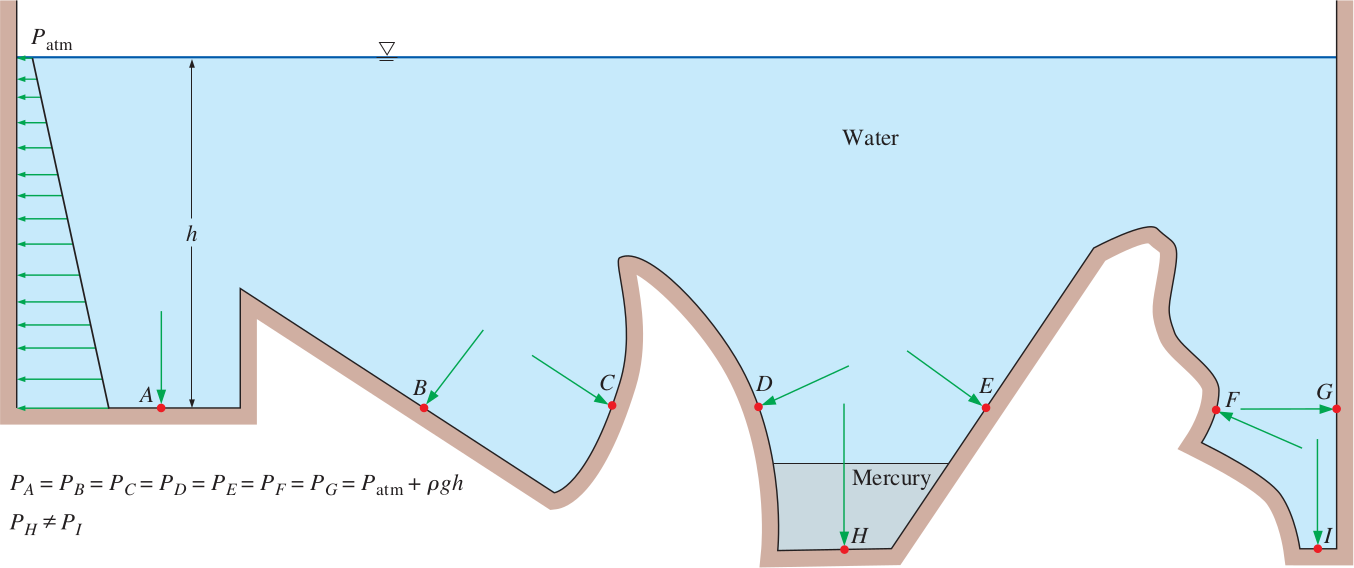
\includegraphics[width=10cm]{pres3}
\caption{Presion sobre puntos sobre superficies de diferentes formas y a diferentes profundidades.}
\label{pres3}
\end{figure}

Como consequencia de que la presion es constante en direccion horizontal, tenemos que \textit{la presion aplicada sobre un fluido confinado en un contenedor, es transmitida igualmente a todas las partes del contenedor y actua perpendicular a las paredes del mismo}. Esto es conocido como la \textbf{Ley de Pascal}. Dicho de otra manera \textit{un cambio en la presion en cualquier punto de un fluido en reposo es transmitido igualmente a todos los puntos del fluido}. La ley de pascal tiene muchas aplicaciones como por ejemplo el sistema de frenos en vehiculos, los elevadores hidraulicos para levantar cargas pesadas, entre otros. Si analisamos la figura~\ref{pres4}, tenemos que $P_1 \ =\ P_2$ ya que estan a un mismo nivel, esto con lleva a la siguiente relacion de fuerzas:

% Fig 3.11 Cengel
\begin{figure}[h]
\centering
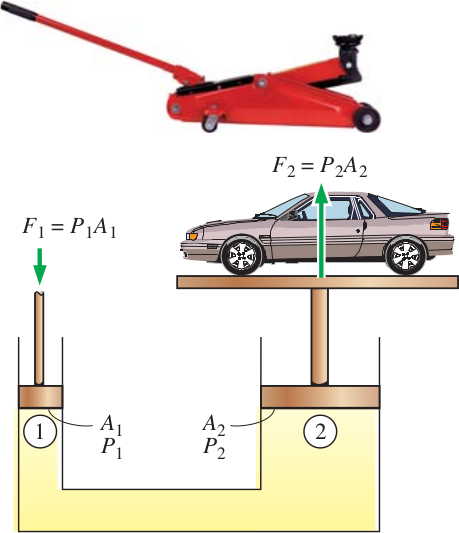
\includegraphics[width=10cm]{pres4}
\caption{Ley de Pascal en un elevador hidraulico.}
\label{pres4}
\end{figure}

\begin{equation}
P_1 = P_2 \quad \rightarrow \quad \frac{F_1}{A_1}=\frac{F_2}{A_2} \quad \rightarrow \quad \frac{F_2}{F_1}=\frac{A_2}{A_1}
\label{ppr6}
\end{equation}

donde la relacion $A_2 / A_1$ es conocida como la \textit{ventaja mecanica} de un elevador hidraulico.

\section{Medidores de presi\'on}
\subsection{Barometro}
La presi\'on atmospherica es medida por un aparato llamado \textbf{barometro} por lo que la presion atmosferica es usualmente conocida como la presion baramometrica. El barometro fue inventado por Evangelista Torricelli (1608-1647) y consiste en invertir un tubo de ensayo lleno de mercurio dentro de un recipiente con mercurio abierto a la atmosfera (ver figura~\ref{baro1}). La presion en el punto B es igual a la presion atmoferica, mientras la presion en el punto C puede considerarse igual zero. Escribiendo el balance de fuerzas sobre la columna de mercurio:

% Fig 3.12 Cengel
\begin{figure}[h]
\centering
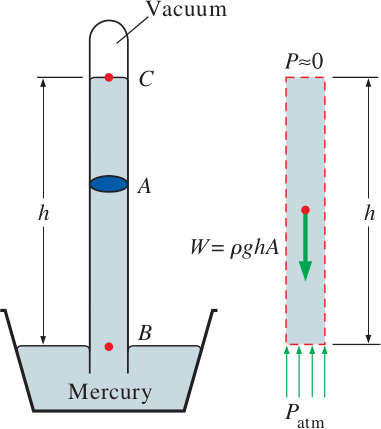
\includegraphics[width=10cm]{baro1}
\caption{El barometro}
\label{baro1}
\end{figure}


\begin{equation}
P = \rho g h
\label{bb1}
\end{equation}
donde $\rho$ es la densidad del mercurio. Note que la altura $h$ de la columns es siempre la misma independiente del diametro del tubo. 

Algunas definiciones:
\begin{itemize}
\item \textbf{atmosfera estandard}: Presion producida por una columna de mercurio de 760 $mm$ de $\rho_{Hg} = 13595\ kg/m^3$ a 0$^oC$ bajo estandard $g=9.807\ m/s^2$. El equivalente en columna de agua seria de 10.3 $m$.
\item \textbf{Torr}: En honor a Torricelli, la unidad $mmHg$ es conocida como $torr$. Por esto, $1\ atm = 760\ torr$ y $1\ torr = 133.3\ Pa$. 
\end{itemize}

Algunas ideas importantes:
\begin{itemize}
\item La $P_{atm}$ disminuye con la altura. Por eso mientras que $P_{atm}=101.325 kPa$, la presion a altitudes como 1000, 2000, 5000 y 10000 y 20000 metros es 89.88, 79.50, 54.05, 26.5 and 5.53 $kPa$, respectivamente.
\item Si $P_{atm}$ depende del peso del aire arriba de una posicion determinada, esta no solo cambia con la altitud, tambien con las condiciones climaticas.
\item Como la temperatura y la presion disminuyen con la altura, cocinar hervir agua en sitios en altas altitudes toma mayor tiempo.
\item Es comun el sangrado nasal en altas altitudes porque la diferencia entre la presion sanguinea y la presion atmosferica se hace mayor por lo que los vasos sanquineos de la nariz son incapaces de soportar este esfuerzo adicional y terminan rompiendose. 
\item Como en altas altitudes la densidad del aire es mas baja, la cantidad de oxigeno por unidad de volumen es menor, por eso nos cansamos mas rapidamente en estos lugares y experimenmos dificultad al respirar.
\end{itemize}

\subsection{El manometro}
De acuerdo con la ecuaci\'on~\ref{ppr1}, el cambio de elevacion $-\Delta z$ en un fluido en reposo es igual a $\Delta P/\rho g$, lo cual sugiere que la columna de un fluido puede ser usada para calcular las diferencias de presion. El \textbf{manometro} es un aparato que esta basado en este principio y por lo tanto es usado para medir differencias de presion. Un manometro es un tubo de plastico o vidrio en forma de U el cual contiene usualmente agua, mercurio, alcohol o aceite (ver figura~\ref{mano1}). Cuando las diferencias de presion son muy  altas, se prefiere un fluido pesado como el mercurio.

\begin{figure}[h]
\centering
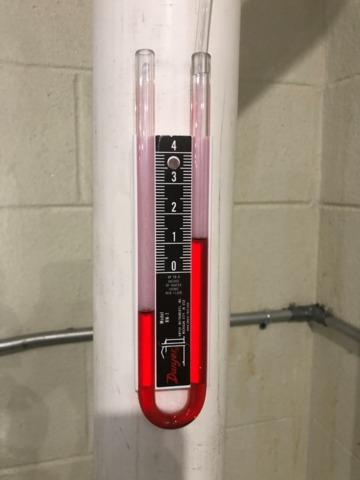
\includegraphics[width=10cm]{mano1}
\caption{Manometro en forma de U}
\label{mano1}
\end{figure}

Consideremos el manometro conectado al tanque con gas de la figura~\ref{mano2}. Teniendo en cuenta que los efectos gravitaciones sobre los gases son despreciables, la presion en cualquier punto del tanque es la misma incluyendo la presion en 1 $P_1$. Se sabe ademas que la presion no varia en direccion horizontal en un fluido, por lo tando, $P_2\ =\ P_1$. Como la altura $h$ de fluido esta en equilibrio estatico y esta abierta a la atmosfera:

% Fig 3.19 Cengel
\begin{figure}[h]
\centering
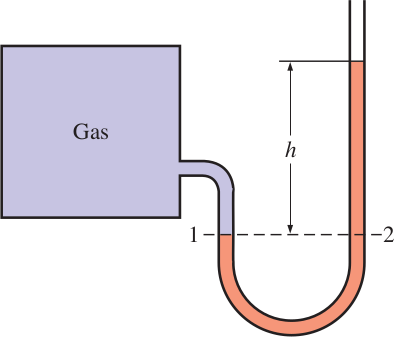
\includegraphics[width=10cm]{mano2}
\caption{Manometro b\'asico.}
\label{mano2}
\end{figure}

\begin{equation}
P_2 = P_{atm} + \rho g h
\label{ma1}
\end{equation}

donde $\rho$ es la densidad del fluido del manometro. A pesar que el area transversal del manometro no cambia $h$, el diametos del tubo debe ser lo suficientemente grande para reducir el efecto capilar.

Algunos problemas en ingenieria involucran manometros con multiples fluidos de diferentes densidades ubicados uno sobre otro. Recuerde que para resolver cualquier problema de manometros:
\begin{enumerate}
\item El cambio de presion en una columna de fluido $h$ es: $\Delta P = \rho gh$.
\item La presion en un fluido incrementa hacia abajo y disminuye hacia arriba ($P_{down} > P_{top}$).
\item Dos puntos conectados por un fluido continuo en reposo sobre el mismo plano horizontal tienen la misma presion. 
\end{enumerate}

Cuando existen differentes tipos de fluidos conectados continuamente y en reposo se puede calcular la presion en un punto determinado partiendo del punto cuya presion es conocida e ir adicionando o substrayendo el termino $\rho g h$ en la direccion al punto de presion desconocida. Por ejemplo si tenemos los fluidos de la figura~\ref{mano3} y queremos calcular la presion en el punto 1, empezamos desde la presion conocida $P_{atm}$ y vamos avanzando hasta el punto 1, lo cual da: 

% Fig 3.21 Cengel
\begin{figure}[h]
\centering
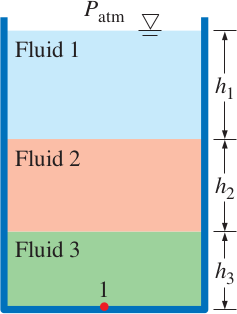
\includegraphics[width=10cm]{mano3}
\caption{Tres tipos de fluido en reposo de diferente $\rho$ ubicados unos sobre el otro.}
\label{mano3}
\end{figure}

$$
P_{atm} + \rho_1 g h_1 + \rho_2 g h_2 + \rho_3 g h_3 = P_1
$$
En el caso en que los tres fluidos tuvieran la misma densidad, la ecuacion anterior quedaria: $P_{atm}+\rho g(h_1 + h_2 + h_3) = P_1$

Los manometros son utilizado para medir los cambios presion (generalmente debido a valvulas o accesorios) entre dos secciones de una tuberia con flujo a presion.  Dicho manometro se conecta entre dos secciones de una tuberia (ver figura~\ref{mano4} que transporta liquido o gas cuya densidad es $\rho_1$. La densidad del liquido en el manometro $\rho_2$ debe ser mayor que $\rho_1$ y ambos fluidos deben ser inmisibles. La diferencia de presion $P_1 - P_2$ puede ser calculada iniciando en el punto 1 y moviendose a lo largo del manometro adicionando o restando $\rho g h$ hasta alcanzar el punto 2, lo cual quedaria:

% Fig 3.22 Cengel
\begin{figure}[h]
\centering
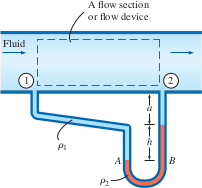
\includegraphics[width=10cm]{mano4}
\caption{Medicion de la diferencia de presion en un tuberia con un manometro.}
\label{mano4}
\end{figure}

$$
P_1 + \rho_1 g (a+h) - \rho_2 g h - \rho_1 ga = P_2
$$
Note que los puntos a una distancia $a$ tienen una misma presion por estar al mismo nivel en el manometro, simplificando:
$$
P_1 - P_2 = (\rho_1 - \rho_2)gh
$$

Si el fluido que fluye a lo largo de la tuberia es gas, $\rho_1 \ll \rho_2$ por lo que la ecuacion anterior se convierte en $P_1-P_2 \cong \rho_2 g h$.


\subsection{Otros medidores de presion}
\begin{itemize}
\item Tubo de Bourdon
\item Transductor de presion
\end{itemize}

\section{Estatica de fluidos}
\end{document}
